\documentclass[12pt]{report}
\usepackage[utf8]{inputenc}
\usepackage[russian]{babel}
%\usepackage[14pt]{extsizes}
\usepackage{listings}
\usepackage{graphicx}
\usepackage{amsmath,amsfonts,amssymb,amsthm,mathtools} 
\usepackage{float}

% Для листинга кода:
\lstset{ %
language=C++,                 % выбор языка для подсветки (здесь это С)
basicstyle=\small\sffamily, % размер и начертание шрифта для подсветки кода
numbers=left,               % где поставить нумерацию строк (слева\справа)
numberstyle=\tiny,           % размер шрифта для номеров строк
stepnumber=1,                   % размер шага между двумя номерами строк
numbersep=5pt,                % как далеко отстоят номера строк от подсвечиваемого кода
showspaces=false,            % показывать или нет пробелы специальными отступами
showstringspaces=false,      % показывать или нет пробелы в строках
showtabs=false,             % показывать или нет табуляцию в строках
frame=single,              % рисовать рамку вокруг кода
tabsize=2,                 % размер табуляции по умолчанию равен 2 пробелам
captionpos=t,              % позиция заголовка вверху [t] или внизу [b] 
breaklines=true,           % автоматически переносить строки (да\нет)
breakatwhitespace=false, % переносить строки только если есть пробел
escapeinside={\#*}{*)}   % если нужно добавить комментарии в коде
}

% Для измененных титулов глав:
\usepackage{titlesec, blindtext, color} % подключаем нужные пакеты
\definecolor{gray75}{gray}{0.75} % определяем цвет
\newcommand{\hsp}{\hspace{20pt}} % длина линии в 20pt
% titleformat определяет стиль
\titleformat{\chapter}[hang]{\Huge\bfseries}{\thechapter\hsp\textcolor{gray75}{|}\hsp}{0pt}{\Huge\bfseries}


% plot
\usepackage{pgfplots}
\usepackage{filecontents}
\usetikzlibrary{datavisualization}
\usetikzlibrary{datavisualization.formats.functions}
\begin{filecontents}{LevR.dat}
100 45504
200 344852
300 1626090
400 4410053
500 8809530
600 15523926
700 27314819
800 36896674
900 151438792
1000 253111941
\end{filecontents}

\begin{filecontents}{LevT.dat}
100 50613
200 254889
300 1164803
400 3277843
500 6466829
600 10441740
700 20235150
800 27982176
900 115139281
1000 199701561
\end{filecontents}

\begin{filecontents}{DamLevR.dat}
100 22663
200 189215
300 937882
400 2605948
500 5077237
600 9041331
700 15047492
800 20829956
900 85256627
1000 158414218
\end{filecontents}



\begin{filecontents}{LevR1.dat}
101 45393
201 386372
301 1557256
401 4538718
501 9009942
601 15214595
701 26603522
801 37648086
901 139235577
1001 278285719
\end{filecontents}

\begin{filecontents}{LevT1.dat}
101 35265
201 364594
301 1113414
401 3314034
501 6511456
601 11947585
701 20274021
801 26844301
901 136919210
1001 212082553
\end{filecontents}

\begin{filecontents}{DamLevR1.dat}
101 38152
201 196174
301 919775
401 2652528
501 5171817
601 10328122
701 15001586
801 20867237
901 108043316
1001 165932409
\end{filecontents}



\begin{document}
%\def\chaptername{} % убирает "Глава"
\begin{titlepage}
	\centering
	{\scshape\LARGE МГТУ им. Баумана \par}
	\vspace{3cm}
	{\scshape\Large Лабораторная работа №6\par}
	\vspace{0.5cm}	
	{\scshape\Large По курсу: "Анализ алгоритмов"\par}
	\vspace{1.5cm}
	{\huge\bfseries Вычислительный конвейер\par}
	\vspace{2cm}
	\Large Работу выполнила: Лаврова Анастасия, ИУ7-55Б\par
	\vspace{0.5cm}
	\LargeПреподаватели:  Волкова Л.Л., Строганов Ю.В.\par

	\vfill
	\large \textit {Москва, 2019} \par
\end{titlepage}

\tableofcontents

\newpage
\chapter*{Введение}
\addcontentsline{toc}{chapter}{Введение}
Целью данной лабораторной работы является применение конвейерной обработки данных. Конвейерная обработка данных может быть полезной,когда каждая операция занимает много времени. В данной работе будет рассмотрена задача "построения автомобиля", а также проведения замера скорости работы работы конвейера при разной нагруженности блоков.


\chapter{Аналитическая часть}
Конвейер - способ организации вычислений, используемый в современных процессорах и контроллерах с целью повышения их производительности (увеличения числа инструкций, выполняемых в единицу времени — эксплуатация параллелизма на уровне инструкций), технология, используемая при разработке компьютеров и других цифровых электронных устройств. \\
Конвейеризация (или конвейерная обработка) в общем случае основана на разделении подлежащей исполнению функции на более мелкие части, называемые ступенями, и выделении для каждой из них отдельного блока аппаратуры. Производительность при этом возрастает благодаря тому, что одновременно на различных ступенях конвейера выполняются несколько команд.\\



\section{Оценка производительности идеального конвейера}

Пусть задана операция, выполнение которой разбито на n последовательных этапов. При последовательном их выполнении операция выполняется за время

\begin{equation}\label{form:way} 
 \tau _{e}={\sum\limits_{i=1}^n \tau _{i}}
 \end{equation}
 \begin{align*}
    \text{где} \\
    n &- \text{количество последовательных этапов;} \\
   \tau _{i} &- \text{время выполнения i-го этапа;}
\end{align*}

Быстродействие одного процессора, выполняющего только эту операцию, составит

\begin{equation}\label{form:way} 
 S_{e}={\frac{1}{\tau _{e}}}={\frac{1}{\sum\limits_{i=1}^n \tau _{i}}}
 \end{equation}
 \begin{align*}
    \text{где} \\
    \tau _{e} &- \text{время выполнения одной операции;} \\
    n &- \text{количество последовательных этапов;} \\
   \tau _{i} &- \text{время выполнения i-го этапа;}
\end{align*}


Максимальное быстродействие процессора при полной загрузке конвейера составляет



Число n — количество уровней конвейера, или глубина перекрытия, так как каждый такт на конвейере параллельно выполняются n операций. Чем больше число уровней (станций), тем больший выигрыш в быстродействии может быть получен.

Известна оценка
\begin{equation}\label{form:way} 
{\frac{n}{n/2} \leq {\frac{S_{max}}{S_{e}}} \leq n}
 \end{equation}
 \begin{align*}
    \text{где} \\
    S_{max} &- \text{максимальное быстродействие процессора  при полной загрузке конвейера;} \\
    S_{e} &- \text{стандартное быстродействие процессора;} \\
   n &- \text{количество этапов.}
\end{align*}

то есть выигрыш в быстродействии получается от n/2  до n раз.

Реальный выигрыш в быстродействии оказывается всегда меньше, чем указанный выше, поскольку:

\begin{enumerate}
\item[1)] некоторые операции, например, над целыми, могут выполняться за меньшее количество этапов, чем другие арифметические операции. Тогда отдельные станции конвейера будут простаивать;
\item[2)] при выполнении некоторых операций на определённых этапах могут требоваться результаты более поздних, ещё не выполненных этапов предыдущих операций. Приходится приостанавливать конвейер;
\item[3)] поток команд(первая ступень) порождает недостаточное количество операций для полной загрузки конвейера.
\end{enumerate}



\chapter{Конструкторская часть}
\textbf{Требования к вводу:}\\
-\\
\textbf{Требования к программе:}\\
Корректная работа конвейера \\


\section{Разработка реализации программы}


Создаются 5 очередей: 3 очереди для 3-х этапов сборки машины, 1 очередь для "пустых"  и 1 очередь для собранных машин.\\
Запускаются потоки для каждой очереди. Функция потока выбирает метод start, который принимает на вход ссылку на следующю очередь. Также функция постоянно ожидает, когда флаг конца работы примет значение True; в противном случае функция проверяет, хранятся ли в очереди необработанные машины. Если остались необработанные машины, то mutex захватывается, достается машина из очереди, mutex освобождается. Начинается обработка машины с помощью функтора work. После выполнения "установки" компонента происходит попытка подключения к очереди следующего этапа конвейера. Ожидается следующая очередь time-for-mutex секунд, если подключиться не удается - засыпаем до тех пор, пока очередь выполнения не опустеет.\\
Если данный этап является "первым" (то есть первым из незавершенных), то назначем следующий этап "первым", а флагу конца работы присваиваем значение True и прекращаем его работу. Если же этот этап не является "первым", то процесс засыпает до тех пор, пока не поступит новая машина, после чего процесс посыпается, обрабатывает очередь, заносит машины в следующую очередь, и так до тех пор, пока этот этап не станет "первым" и не отработает до конца, после этого к нему мы больше не будем возвращаться.\\

На рис. 2.1 представлена схема установки компонента в машину:
	\begin{figure}[h]
        	\begin{center}
        		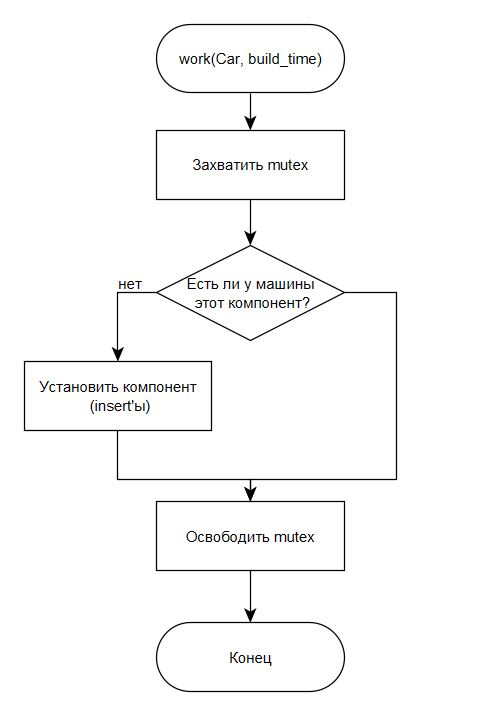
\includegraphics[scale=0.7]{1}
        		\caption{Схема установки компонента в машину}
        		\label{fig:def}
        	\end{center}
        \end{figure}

На рис. 2.2 представлена схема работы одного этапа конвейера:
	\begin{figure}[h]
        	\begin{center}
        		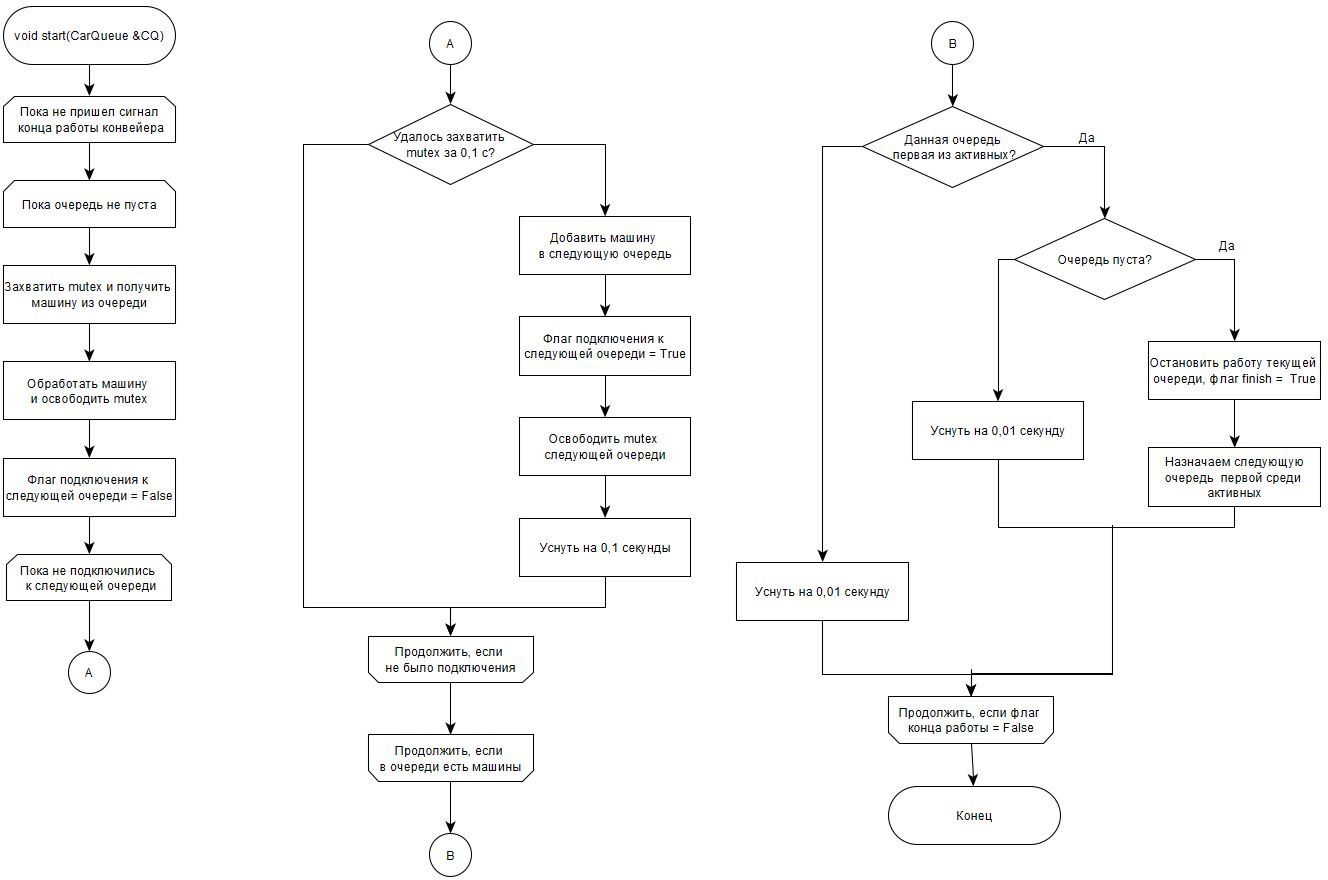
\includegraphics[scale=0.63]{2_1}
        		\caption{Схема работы одного этапа конвейера}
        		\label{fig:def}
        	\end{center}
        \end{figure}


\chapter{Технологическая часть}
\section{Выбор ЯП}
Для реализации программ я выбрала язык программирования C++, так имею большой опыт работы с ним. Среда разработки - Visual Studio. \\

Для работы с потоками и мьютексами применялись библиотеки windows.h(для сна Sleep), mutex, thread. Контейнером очереди был std::queue, поэтому также использовалась библиотека queue. \\

Для замера процессорного времени используется функция, возвращающая количество тиков.\\

"Машина" состоит из трёх компонентов: корпуса, двигателя и электроники. Один из трёх этапов сброки представлен классом CarQueue, который хранит следующие поля:
	\begin{enumerate}
	\item[1)] cars - очередь машин, ожидающих выполнения действия
    \item[2)] work - функтор - функция постройки
    \item[3)] queue\_mutex - временной(для установки времени ожидания) мьютекс для блокировки доступа к очереди выполнения
    \item[4)] main - флаг первой активной очереди
    \item[5)] build\_time - время постройки
    \item[6)] downtime - время ожидания появления элементов в очереди
    \item[7)] time\_for\_mutex - время ожидания на мьютексе
    \item[8)] id - идентификатор танка для отладки
    \end{enumerate}

\begin{lstlisting}[label=some-code,caption=Функция получения тиков]
unsigned __int64 tick() 
{ 
	return (__rdtsc()); 
}

\end{lstlisting}

\section{Реализация вычислительного конвейера}

\begin{lstlisting}[label=s,caption= Функция start]
void CarQueue::start(CarQueue &TQ) {
	finish_mutex.lock();

	while (!finish) {
		finish_mutex.unlock();
		queue_mutex.lock();
		while (Cars.size() > 0) {
			times_in.push_back(clock());
			Car Car = pop();
			queue_mutex.unlock();
			Car = work(Car, build_time);
			bool connect = 0;
			while (!connect) {
				if (TQ.queue_mutex.try_lock_for(
					Ms(time_for_mutex))) {
					TQ.push(Car);
					times_out.push_back(clock());
					connect = 1;
					TQ.queue_mutex.unlock();
				}
				std::this_thread::sleep_for(Ms(50));
			}
			queue_mutex.lock();
		}
		queue_mutex.unlock();
		main_mutex.lock();
		if (main && Cars.size() == 0) {
			main_mutex.unlock();

			finish_mutex.lock();
			finish = 1;
			finish_mutex.unlock();

			TQ.main_mutex.lock();
			TQ.set_main();
			TQ.main_mutex.unlock();


			end = clock();
		}
		else {
			main_mutex.unlock();
			std::this_thread::sleep_for(Ms(downtime));
		}
		finish_mutex.lock();
	}
	finish_mutex.unlock();
}
\end{lstlisting}

	\begin{lstlisting}[label=p,caption=Функция add-engine - встроить двигатель]
Car add_engine(Car &Car, DWORD time) {
	Car.Car_mutex.lock();

	if (!Car.has_engine()) {
		Engine engine;
		Car.insert_engine(engine, time);
	}

	Car.Car_mutex.unlock();

	return Car;
}
\end{lstlisting}


	\begin{lstlisting}[label=pf,caption=Функция add-electronics - встроить электронику]
Car add_Electronics(Car &Car, DWORD time) {
	Car.Car_mutex.lock();

	if (!Car.has_Electronics()) {
		Electronics Electronics;
		Car.insert_Electronics(Electronics, time);
	}

	Car.Car_mutex.unlock();

	return Car;
}
\end{lstlisting}

	\begin{lstlisting}[label=pf,caption=Функция add-body - встроить корпус]
Car add_body(Car &Car, DWORD time) {
	Car.Car_mutex.lock();

	if (!Car.has_body()) {
		Body body;
		Car.insert_body(body, time);
		std::cout << "\n add body to Car " << Car.id;
	}
	Car.Car_mutex.unlock();
	return Car;
}
\end{lstlisting}

	\begin{lstlisting}[label=pf,caption=Функция main]
int main()
{
	Car::count = 1;
	CarQueue::count = 1;

	size_t amount = 5;
	CarQueue Cars(amount);

	CarQueue queue_engine(add_engine, 90);
	CarQueue queue_body(add_body, 30);
	CarQueue queue_weapon(add_Electronics, 200);

	CarQueue ready_Cars;

	std::thread give_to_body([&Cars, &queue_body]() { Cars.start(queue_body); });
	std::thread give_to_engine([&queue_body,
		&queue_engine]() {
		queue_body.start(queue_engine);
	});

	std::thread give_to_weapon([&queue_engine,
		&queue_weapon]() {
		queue_engine.start(queue_weapon);
	});

	std::thread give_to_ready([&queue_weapon,
		&ready_Cars]() {
		queue_weapon.start(ready_Cars);
	});

	give_to_body.join();
	give_to_engine.join();
	give_to_weapon.join();
	give_to_ready.join();

	std::cout << "\n\ni finished! " << ready_Cars.size() << " " << queue_weapon.size() << queue_engine.size() << queue_body.size();

	return 0;
}
\end{lstlisting}


	\begin{lstlisting}[label=pf,caption=Функция CarQueue - конструктор класса для пустой очереди]
CarQueue::CarQueue(size_t amount) {
	end = begin = clock();
	id = CarQueue::count++;
	for (size_t i = 0; i < amount; i++) {
		Car Car;
		Cars.push(Car);
	}
	main = 1;
	finish = 0;
	work = noWork;
	time_for_mutex = 100;
	downtime = 100;
}
\end{lstlisting}

	\begin{lstlisting}[label=pf,caption= Конструктор класса для очереди построения компонента]
CarQueue::CarQueue(std::function<Car(Car&, DWORD)> f, DWORD t) {
	end = begin = clock();
	id = CarQueue::count++;
	main = 0;
	finish = 0;
	work = f;
	build_time = t;
	time_for_mutex = 100;
	downtime = 100;
}
\end{lstlisting}

	\begin{lstlisting}[label=pf,caption= Конструктор копирования]
CarQueue::CarQueue(const CarQueue & other) {
	id = other.id;
	Cars = other.Cars;
	work = other.work;
	finish = other.finish;
	main = other.main;
	time_for_mutex = other.time_for_mutex;
	downtime = other.downtime;
}
\end{lstlisting}

	\begin{lstlisting}[label=pf,caption=  Конструктор перемещения]
CarQueue::CarQueue(const CarQueue && other) {
	id = other.id;
	Cars = other.Cars;
	work = other.work;
	finish = other.finish;
	main = other.main;
	time_for_mutex = other.time_for_mutex;
	downtime = other.downtime;
}
\end{lstlisting}




\chapter{Исследовательская часть}

\section{Постановка эксперимента}

Был проведен сравнительный анализ реализаций конвейера при разной нагруженности этапов конвейера. Замеры времени проводились для 10 элементов. Идеальное время сборки машины - 3 секунды.\\
Проведены 3 опыта, в каждом из которых время одного этапа оставалось неизменным (равное 1000 мс), а время двух других этапов варьировалось.\\
Последний - четвертый, - опыт показывает пример работы конвейера с наибольшей и наименьшей разницей между этапами.\\
В результате получается, что последний столбец отражает суммарное время работы,  так как третий этап конвейера запускается в то же время, что и самый первый, а заканчивается самым последним.



\centering  
\begin{tikzpicture}
	\begin{axis}[
		    xlabel={Разница времени выполнения частей конвейера},
		    ylabel={Время в милисекундах},
		    ymin = 7000, ymax = 22000,
		    legend pos=north west,
		    ymajorgrids=true,
		    grid style=dashed,
		]
		\legend{ 
	        Опыт 1,
	        Опыт 2,
	        Опыт 3,
	        Наилучший и наихудший случай
	        }
  		\addplot[
  		    color=blue,
  		    mark=square,
  		    ]
  		    coordinates {
  		    (200,  7916)
  		    (600,  8717)
  		    (1000, 9510)
  		    (1400, 10313)
			(1800, 11111)
  		    };
  		\addplot[
  		    color=red,
  		    mark=square,
  		    ]
  		    coordinates {
  		    (200,  7920)
  		    (600,  8716)
  		    (1000, 9520)
  		    (1400, 10310)
			(1800, 11121)
  		    };
  		\addplot[
  		    color=yellow,
  		    mark=square,
  		    ]
  		    coordinates {
  		    (200,  7910)
  		    (600,  8712)
  		    (1000, 9510)
  		    (1400, 10317)
			(1800, 11118)
  		    };
  		\addplot[
  		    color=green,
  		    mark=square,
  		    ]
  		    coordinates {
  		    (2700,  14709)
  		    (0   ,  7511)
  		    };
		\end{axis}
	\end{tikzpicture}
       
	

\begin{table}[h!]
        \caption{Зависимость времени работы конвейера от разницы времени работы отдельных его составляющих}
            \begin{tabular}{ | c | c | c | c | c | c | }
                \hline
                 Время   &  Время   &  Время  &  Суммарное  & Суммарное  & Суммарное \\
                 одного   &  одного   &  одного  &  время & время &  время \\
                 выполнения   &  выполнения   &  выполнения  & работы & работы & работы  \\ 
                  первого  & второго  & третьего  & работы  & работы & работы  \\ 
                 этапа & этапа & этапа & 1 этапа & 2 этапа & 3 этапа  \\ 
                 (в мс) & (в мс) & (в мс) & (в мс) & (в мс) & (в мс)  \\ 
                 \hline  
                900 & 1100 & 1000 & 5005 & 6906 & 7916  \\
                700 & 1300 & 1000 & 4005 & 7711 & 8717  \\
                500 & 1500 & 1000 & 3006 & 8509 & 9510  \\
                300 & 1700 & 1000 & 2004 & 9311 & 10313 \\
                100 & 1900 & 1000 & 1008 & 10108& 11111 \\
                
                1100 & 1000 & 900 & 6006 & 7013 & 7920  \\
                1300 & 1000 & 700 & 7005 & 8011 & 8716  \\
                1500 & 1000 & 500 & 8005 & 9015 & 9520  \\
                1700 & 1000 & 300 & 9004 & 10008& 10310 \\
                1900 & 1000 & 100 & 10005& 11014& 11121 \\
                
                1000 & 900 & 1100 & 5505 & 6407 & 7910  \\
                1000 & 700 & 1300 & 5507 & 6212 & 8712  \\
                1000 & 500 & 1500 & 5505 & 6011 & 9510  \\
                1000 & 300 & 1700 & 5507 & 5813 & 10317 \\
                1000 & 100 & 1900 & 5505 & 5610 & 11118 \\
                
                100  & 100 & 2800 & 1005 & 1107 & 14709 \\
                1000 & 1000& 1000 & 5505 & 6509 & 7511  \\
                2800 & 100 & 100  & 14505& 14611& 14715 \\
               
                \hline
            \end{tabular}
        \label{tab:a_b_c}
    \end{table} 
	

        \newpage    
 

\section{Вывод}

Эксперименты показали, что конвейер работает наиболее быстро, когда время работы каждого из его составляющих примерно одинаково. 


\chapter*{Заключение}
\addcontentsline{toc}{chapter}{Заключение}
В ходе работы был изучаен и реализован вычислительный конвейер из трёх этапов. Были определены наиболее оптимальные параметры для быстрого решения.



\end{document}